\documentclass[twoside]{article}
\input{ISC18-english.sty}
%%%%%%%%%%%%%%%%%%%%%%%%%%%%  Make sure to compile twice for proper cross-references. %%%%%%%%%%%%%%%%%%%%%%%
%%%%%%% For proper display of references, compile the document twice. %%%%%%%%%%%%%%%%%%%%%
%%%%%%%%%%%%%%% If using TeX Live, compile using pdflatex command %%%%%%%%%%%%%%%%%%%%%%%

\begin{document}
\thispagestyle{empty}
%%%%%%%%%%%%%%%%% Article title header  %%%%%%%%%%%%%%%%%%%%
\fancyhead[LE]{Order Statistics in R}
%%%%%%%%%%%%%%%%% Article authors header   %%%%%%%%%%%%%%%%%%%%
\fancyhead[RO]{M. Salehi and R. Arafeh}
\begin{center}
{
\includegraphics [height=25mm, width=150.3mm] {Images/isc18E}} \\
\vspace*{-1.8cm}
%\begin{center}
%\color{blue} 
%{\hspace{0.1cm}\rule{\textwidth}{1mm}}\\
%\end{center}
\vspace*{4cm}
%%%%%%%%%%%%%%%%% Article title  %%%%%%%%%%%%%%%%%%%%
{\Large \bf Order Statistics in R: Moment Computation, Goodness-of-Fit Assessment, and Statistical Inference with the $\mathsf{mos}$ Package}\\
%%%%%%%%%%%%%%%%% Article authors and affiliations %%%%%%%%%%%%%%%%%%%%
{\bf
Mahdi Salehi\footnote[1]{{\bf Corresponding Author:} {\tt salehi.sms@neyshabur.ac.ir }} and Reyhaneh Arafeh$^2$\\
$^1$Department of Mathematics and Statistics, University of Neyshabur, Iran \\
$^2$Depatment of Statistics, Ferdowsi University of Mashhad, Iran}

\end{center}
\rule{\textwidth}{0.2mm}\\
%%%%%%%%%%%%%%%%% Article abstract  %%%%%%%%%%%%%%%%%%%%
\noindent{\bf Abstract:}\\
Although order statistics are fundamental in statistical inference, reliability analysis, and goodness-of-fit assessment, computational tools for their moment evaluation remain limited. In this paper, we briefly  introduce the \textsf{R} package $\mathsf{mos}$ which provides a unified framework for the analysis of order statistics, censored samples, and $k$-record values. The package combines analytical evaluation of moments, whenever closed-form expressions are available, with Monte Carlo estimation for more general distributions. It also provides functions for variance, skewness, kurtosis, and efficient simulation of ordered-data structures. Applications to graphical goodness-of-fit diagnostics and best linear unbiased estimation illustrate the practical utility of the package. The $\mathsf{mos}$ offers a consistent and extensible environment for research and applications involving ordered data.

\noindent{\bf Keywords:}
Censoring, Order statistics, Moments, Record values, Reliability, R programming language. \\
\noindent{\bf Mathematics Subject Classification (2010):} $\rm 62G30$, $\rm 62$-$\rm 04$, $\rm 62N05$. \\
\hspace{1cm}\rule{\textwidth}{0.2mm}\\

%% ===========================================================================
\section{Introduction}\label{sec:intro}
%% ===========================================================================
Order statistics, obtained by arranging a random sample $X_1,\ldots,X_n$ in
non-decreasing order as $X_{1:n}\le\cdots\le X_{n:n}$,
are fundamental in statistical theory and applications. They support extreme-value analysis through sample minima and maxima, provide robust estimators such as medians and trimmed means, and naturally arise in reliability and survival data settings \citep{DavidNagaraja2003}. Closely related data structures include censored samples, in which only partial order information is available under schemes such as Type-I, Type-II, or progressive censoring, and record values, which arise as successive extremes in sequential observations and naturally extend to $k$-record processes.
A central computational challenge in working with order statistics is the evaluation of their moments. Single and product moments are essential in methods such as best linear unbiased estimation (BLUE), $L$-moments
and goodness-of-fit procedures \citep{ArnoldBalakrishnanNagaraja2008}. While closed-form expressions exist for several parent distributions, they are scattered across the literature and lack a unified computational implementation. For many commonly used distributions, such expressions are unavailable, and simulation-based approximations are required.

Several R packages address individual components of this workflow. Existing tools provide functionality for generating order statistics, handling censored data, or computing $L$-moments. However, most focus on isolated tasks. To the best of our knowledge, no existing package provides a unified framework that integrates analytical and simulation-based computation of general order-statistic moments with tools for censored samples and record-value generation within a single coherent interface.
The $\mathsf{mos}$ package \citep{mos}, provides a unified computational framework for order-statistic analysis. It implements both analytical and simulation-based computation of moments, depending on the availability of closed-form expressions in the literature. The package further offers tools for deriving higher-order summaries such as variance, skewness, and kurtosis, and includes efficient simulation routines for order statistics, censored samples, and $k$-record values within a consistent interface.

The remainder of the paper is organized as follows. Section~\ref{sec:design} describes the computational framework of package. Section~\ref{sec:usage} illustrates usage examples, and Section~\ref{sec:application} presents applications to goodness-of-fit assessment and statistical inference. Section~\ref{sec:summary} concludes the paper.
%% ===========================================================================
\section{Computational framework of the $\mathsf{mos}$ package}\label{sec:design}
Let $X_1,\ldots,X_n$ be a continuous random sample drawn from a cumulative distribution function (cdf) $F$ with density
$f$, and let $X_{r:n}$ denote the $r$th order statistic. Its $k$th single moment \citep{DavidNagaraja2003}
is
\begin{equation*}\label{eq:single-moment}
  \mu_{r:n}^{(k)} = \mathbb{E}\!\left[X_{r:n}^{k}\right]
  = r \binom{n}{r}\int_{-\infty}^{\infty} x^{k}\,[F(x)]^{r-1}[1-F(x)]^{n-r} f(x)\,\mathrm{d}x
\end{equation*}
The $\mathsf{mos}$ exposes
$\mu_{r:n}^{(k)}$ through the \texttt{mo\_*()} functions  using a \emph{dual framework}: whenever a tractable closed form is
available it is evaluated directly (deterministic and fast), and otherwise the
moment is estimated by Monte Carlo.
Closed forms are used for the uniform, exponential, Weibull, symmetric
triangular, Topp--Leone and complementary beta distributions (with references in
Table~\ref{tab:functions}); Monte Carlo is used for the normal, Student~$t$,
gamma, beta, Pareto and Kumaraswamy \citep{Kumaraswamy1980} parents, with defaults
$M=10^{5}$ replicates and \texttt{seed = 42}. The variance, skewness and the
Pearson measures of kurtosis of $X_{r:n}$ follow from the first four single
moments and are returned by
\texttt{varOS()}, \texttt{skewOS()} and \texttt{kurtOS()}. Table~\ref{tab:functions}
summarizes the exported functions.

\begin{table}[h]
\begin{center}
\small
\caption{\label{tab:functions}Main exported functions of $\mathsf{mos}$. The
analytical \texttt{mo\_*()} functions evaluate closed-form moments from the cited
sources; the remaining \texttt{mo\_*()} functions use Monte Carlo.}
\begin{tabular}{|l|l|}
  \hline
Function & Purpose \\  \hline \hline
\texttt{ros()} & Simulates order statistics (single or several ranks) \\
\texttt{rcens()} & Simulates Type-I and Type-II censored samples \\
\texttt{rpcens2()} & Simulates progressive Type-II censored samples \\
\texttt{rkrec()} & Simulates first upper / lower $k$-record values \\
\hline
\texttt{mo\_unif()} & Uniform moments \citep{ArnoldBalakrishnan2012} \\
\texttt{mo\_exp()} & Exponential moments \citep{Ahsanullah2013} \\
\texttt{mo\_weibull()} & Weibull moments \citep{HarterBalakrishnan1996} \\
\texttt{mo\_tri()} & Symmetric triangular moments \citep{Nagaraja2013} \\
\texttt{mo\_topple()} & Topp--Leone moments \citep{Genc2012} \\
\texttt{mo\_compbeta()} & Complementary beta moments \citep{Jones2002,Makouei2021} \\
\texttt{mo\_norm()}, \texttt{mo\_t()}, \texttt{mo\_gamma()}, & \\
\texttt{mo\_beta()}, \texttt{mo\_pareto()}, \texttt{mo\_kumar()} & Normal, $t$, gamma, beta, Pareto, Kumaraswamy (Monte Carlo) \\
\hline
\texttt{varOS()}, \texttt{skewOS()}, \texttt{kurtOS()} & Variance, skewness, kurtosis of $X_{r:n}$ \\  \hline
\end{tabular}
\end{center}
\end{table}

All simulation rests on the generator \texttt{ros()}. Since
$F(X_{r:n})\sim\mathrm{Beta}(r,n-r+1)$ for any continuous $F$, a single rank is
drawn as $F^{-1}(B)$ with $B\sim\mathrm{Beta}(r,n-r+1)$---one beta draw and one
quantile evaluation, with no sorting---so order statistics can be generated from
any continuous distribution with a known quantile function, built in or supplied
through \texttt{qf}; for several ranks \texttt{ros()} generates, sorts and subsets
complete samples to preserve their joint distribution. $\mathsf{mos}$ also supports
two related ordered-data structures. \emph{Censored samples}
\citep{BalakrishnanAggarwala2000} arise in life-testing: Type-I stops the test at a
fixed time $T$, Type-II at the $r$th failure (the first $r$ order statistics), and
progressive Type-II withdraws $R_i$ surviving units at the $i$th failure for a
scheme $R=(R_1,\ldots,R_m)$ with $m+\sum_i R_i=n$; these are simulated by
\texttt{rcens()} and \texttt{rpcens2()} (the latter using the algorithm of
\citep{BalakrishnanSandhu1995}). \emph{$k$-record statistics}
\citep{ArnoldBalakrishnanNagaraja1998} generalize ordinary records by tracking the
$k$th largest value seen so far (the case $k=1$ is the usual record); the first
upper and lower $k$-record values are generated by \texttt{rkrec()}.

%% ===========================================================================
\section{Using the package}\label{sec:usage}
The generator \texttt{ros()} simulates order statistics: a scalar \texttt{r}
returns one rank and a vector \texttt{r} a matrix preserving their joint
distribution. It also accepts a user-defined quantile function through the
\texttt{qf} argument, so order statistics can be drawn from any continuous
distribution. The \texttt{mo\_*()} functions return single moments through a
common interface (deterministic for the analytical families, Monte Carlo
otherwise), and \texttt{varOS()}, \texttt{skewOS()}, \texttt{kurtOS()} return the
corresponding summaries:
\par\smallskip
\begin{verbatim}
> set.seed(1)
> ros(5, r = 2, n = 10, dist = "norm")
[1] -1.238927 -0.808177 -1.348781 -0.726418 -1.340785
> qgompertz <- function(p, a, b) log(1 - log(1 - p) * b / a) / b
> set.seed(2)
> ros(5, r = 3, n = 8, qf = "qgompertz", a = 1, b = 2)  # user quantile fn
[1] 0.1760290 0.3252047 0.1487873 0.2850333 0.3170499
> mo_unif(r = 2, n = 5, k = 1)   # closed form = r/(n+1) = 1/3
[1] 0.333333
> mo_norm(r = 2, n = 10, k = 4)  # Monte Carlo
[1] 2.549317
\end{verbatim}
\par\smallskip
Censored samples and $k$-record values are generated analogously through
\texttt{rcens()}, \texttt{rpcens2()} and \texttt{rkrec()}; for example, a
progressive Type-II sample with scheme $R=(2,1,2,0,0)$:
\par\smallskip
\begin{verbatim}
> set.seed(1)
> rpcens2(n = 10, R = c(2, 1, 2, 0, 0), dist = "exp", rate = 1)
[1] 0.1601063 0.1738609 0.2852860 0.7795502 2.1056580
\end{verbatim}

\section{Application}
\label{sec:application}
%% ===========================================================================
We illustrate two applications of order-statistic moments computed with $\mathsf{mos}$: a
graphical goodness-of-fit diagnostic for the complementary beta distribution
(Section~\ref{sec:app-gof}), and best linear unbiased estimation of location and
scale parameters (Section~\ref{sec:app-blue}).
\subsection{Goodness-of-fit for the complementary beta distribution}
\label{sec:app-gof}
Expected order-statistic values furnish a graphical goodness-of-fit
diagnostic for distributions, as exploited by
\cite{Makouei2021}. More specifically, for an ordered sample $x_{(1)}\le\cdots\le x_{(n)}$ one plots
the estimated values of $\mathbb{E}[X_{i:n}]$ against the sorted observations $x_{(i)}$.
Under a well-fitting model, the points lie near the identity line, whereas
systematic departures indicate lack of fit. We reproduce the flood-levels
application of \cite{Makouei2021} using $\mathsf{mos}$.

The data are the maximum flood levels (in millions of cubic feet per second) of
the Susquehanna River at Harrisburg, Pennsylvania, over twenty four-year periods
from 1890 to 1969:

\begin{verbatim}
> flood <- c(0.654, 0.613, 0.315, 0.449, 0.297, 0.402, 0.379, 0.423,
+             0.379, 0.324, 0.269, 0.740, 0.418, 0.412, 0.494, 0.416,
+             0.338, 0.392, 0.484, 0.265)
\end{verbatim}
\par\smallskip
Following \cite{Makouei2021}, the complementary beta (CB) distribution is
compared with the beta and Kumaraswamy (Kw) distributions, using their
$L$-moment parameter estimates (Table~\ref{tab:flood-fit}). For each model the
expected means $\mathbb{E}[X_{i:n}]$, $i=1,\ldots,20$, are computed with
\texttt{mo\_compbeta()} (closed form, CB), \texttt{mo\_beta()} and
\texttt{mo\_kumar()} (Monte Carlo).

\begin{table}[h]
\begin{center}
\small
\caption{\label{tab:flood-fit}{\small The $L$-moment parameter estimates and goodness of fit 
criteria associated with the Susquehanna River flood-levels data computed using the $\mathsf{mos}$ packages, as reported by 
\cite[Table~8]{Makouei2021}.}}
\begin{tabular}{|c|cccccc|}
  \hline
Model & $\hat a$ & $\hat b$ & KS p-value & KS test statistic & AD p-value & AD test statistic\\  \hline \hline
CB & 0.22 & 0.16 & 0.475 & 0.189 & 0.593 & 0.685\\
Beta & 6.69 & 9.12 & 0.466 & 0.189 & 0.559 & 0.696\\
Kw & 1.67 & 3.21 & 0.045 & 0.307 & 0.067 & 2.247\\  \hline
\end{tabular}
\end{center}
\end{table}

Figure~\ref{fig:gofflood} plots the expected means against the sorted
data for all three models.
Plotting them against the sorted data, the CB and
beta points cluster on the identity line whereas the Kw points depart from it in
the lower tail, agreeing with the KS and AD tests given by \cite{Makouei2021}. 

\begin{figure}[ht]
\begin{center}
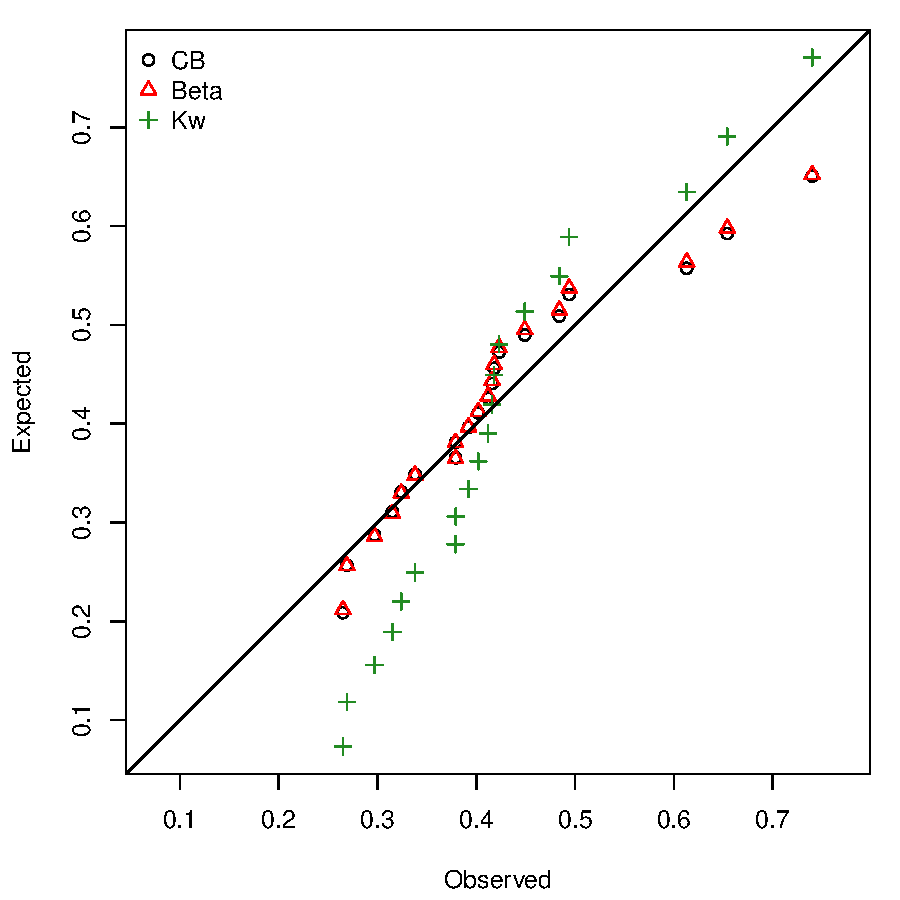
\includegraphics[height = 7cm, width=8cm]{Images/gof_flood.pdf}\\
\vspace{-0.2cm}
\caption{\label{fig:gofflood}\footnotesize{Expected order-statistic means $\mathbb{E}[X_{i:20}]$,
$i=1(1)20$, versus the sorted Susquehanna River flood-levels data.}}
\end{center}
\end{figure}


\subsection{Best linear unbiased estimation of location and scale}
\label{sec:app-blue}
A classical use of order-statistic moments is the construction of best linear
unbiased estimators (BLUEs) of the location and scale parameters of a
location--scale family based on its order statistics, i.e.   $X_{i:n}=\mu+\sigma Z_{i:n}$, where $Z$ is the standardized
parent. Writing $\boldsymbol\alpha=\mathbb{E}[\mathbf Z]$ for the vector of
standardized order-statistic means, $\boldsymbol\Sigma=\mathrm{Cov}(\mathbf Z)$ for
their covariance matrix, and $\mathbf X=(X_{1:n},\ldots,X_{n:n})^{\!\top}$, the
BLUEs of the location and scale parameters are respectively obtained as \citep{Lloyd1952, BalakrishnanLi2008}
\begin{equation}\label{eq:blue}
  \hat\mu = -\boldsymbol\alpha^{\!\top}\boldsymbol\Gamma\,\mathbf X,
  \qquad
  \hat\sigma = \mathbf 1^{\!\top}\boldsymbol\Gamma\,\mathbf X,
  \qquad
  \boldsymbol\Gamma=
  \frac{\boldsymbol\Sigma^{-1}
  (\mathbf 1\boldsymbol\alpha^{\!\top}-\boldsymbol\alpha\mathbf 1^{\!\top})
  \boldsymbol\Sigma^{-1}}
  {(\mathbf 1^{\!\top}\boldsymbol\Sigma^{-1}\mathbf 1)
   (\boldsymbol\alpha^{\!\top}\boldsymbol\Sigma^{-1}\boldsymbol\alpha)
   -(\mathbf 1^{\!\top}\boldsymbol\Sigma^{-1}\boldsymbol\alpha)^{2}},
\end{equation}
where $\mathbf 1$ is the vector of ones. The inputs $\boldsymbol\alpha$ and
$\boldsymbol\Sigma$ are exactly the order-statistic moments $\mathsf{mos}$ delivers:
the means $\boldsymbol\alpha$ from the \texttt{mo\_*()} functions and the variances
$\mathrm{Var}(Z_{r:n})$ on the diagonal of $\boldsymbol\Sigma$ from
\texttt{varOS()}; since product moments are not yet implemented, the off-diagonal
covariances are obtained by simulating the full ordered sample with
\texttt{ros()}.

We illustrate this using the remission times (in years) of $20$ leukemia patients, modelled by a two-parameter exponential distribution as in \citet{Barakat2021}, where a Kolmogorov--Smirnov test indicates a good fit ($D=0.103$, $p=0.97$). 
The quantities required for linear estimation are obtained directly from $\mathsf{mos}$: expected order statistics via \texttt{mo\_exp()}, variances via \texttt{varOS()}, and covariances through simulation with \texttt{ros()}. These moments can then be assembled to construct the BLUEs of the location and scale parameters.
For the two-parameter exponential distribution, the BLUEs are also available in closed form \citep{ArnoldBalakrishnanNagaraja2008}
\[
\hat{\mu}=\frac{nX_{1:n}-\bar X}{n-1}, 
\qquad
\hat{\sigma}=\frac{n(\bar X-X_{1:n})}{n-1},
\]
providing a convenient benchmark against which the moment-based estimates can be compared. Applying both approaches to the leukemia data yields identical estimates,
$\hat{\mu}=0.95$ and
$\hat{\sigma}=1.24$,
with any negligible discrepancies attributable to Monte Carlo error in the simulated covariance matrix. In contrast, the ordinary sample mean $\bar X=2.19$ estimates $\mu+\sigma$ rather than the location parameter $\mu$ and is not consistent for $\mu$, illustrating the advantage of BLUE-based inference for this asymmetric family. 
This example shows how the moment-computation core of
$\mathsf{mos}$---means from \texttt{mo\_exp()}, variances from \texttt{varOS()}, and
covariances via \texttt{ros()}---feeds directly into classical linear estimation;
built-in BLUE support and product moments are a natural direction for further
development.


%% ===========================================================================
\section{Discussion}\label{sec:summary}
%% ===========================================================================
The $\mathsf{mos}$ package unifies the moments computation and simulation of order statistics, censored samples, and $k$-record values within a single framework. By combining exact formulas with Monte Carlo methods, it supports both theoretical investigations and practical data analysis. Future work will focus on product moments, direct covariance computation, and dedicated routines for BLUE and related inferential procedures.

%% -- Bibliography ------------------------------------------------------------


\begin{thebibliography}{99}
\bibitem[Ahsanullah et al.(2013)]{Ahsanullah2013}
Ahsanullah M., Nevzorov V.B. and Shakil M. (2013), {\it An Introduction to Order Statistics,} Paris, Atlantis Press.

\bibitem[Arafeh and Salehi(2025)]{mos}
Arafeh R. and Salehi M.(2025), $\mathsf{mos}$: Simulation and Moment Computation for Order Statistics, R package version 0.1.3, URL \url{https://CRAN.R-project.org/package=mos}.

\bibitem[Arnold and Balakrishnan(2012)]{ArnoldBalakrishnan2012}
Arnold B.C. and Balakrishnan N. (2012), {\it Relations, Bounds and Approximations for Order Statistics,} New York, Springer.

\bibitem[Arnold et al.(1998)]{ArnoldBalakrishnanNagaraja1998}
Arnold B.C., Balakrishnan N. and Nagaraja H.N. (1998), {\it Records,} New York, John Wiley \& Sons.

\bibitem[Arnold et al.(2008)]{ArnoldBalakrishnanNagaraja2008}
Arnold B.C., Balakrishnan N. and Nagaraja H.N. (2008), {\it A First Course in Order Statistics,} Philadelphia, SIAM.

\bibitem[Balakrishnan and Aggarwala(2000)]{BalakrishnanAggarwala2000}
Balakrishnan N. and Aggarwala R. (2000), {\it Progressive Censoring: Theory, Methods, and Applications,} Boston, Birkh\"auser.

\bibitem[Balakrishnan and Sandhu(1995)]{BalakrishnanSandhu1995}
Balakrishnan N. and Sandhu R.A. (1995), A simple simulational algorithm for generating progressive Type-II censored samples, {\it The American Statistician} 49(2), 229--230.

\bibitem[Balakrishnan and Li(2008)]{BalakrishnanLi2008}
Balakrishnan, N. and Li, T. (2008),
Ordered ranked set samples and applications to inference, \textit{Journal of Statistical Planning and Inference}, 138, 3512--3524.

\bibitem[Barakat et al.(2021)]{Barakat2021}
Haroon M. Barakat and Osama M. Khaled and Hadeer A. Ghonem (2021), New Method for Prediction of Future Order Statistics, {\it Quality Technology \& Quantitative Management} 18(1), 101--116.

\bibitem[David and Nagaraja(2003)]{DavidNagaraja2003}
David H.A. and Nagaraja H.N. (2003), {\it Order Statistics,} 3rd ed., Hoboken, John Wiley \& Sons.

\bibitem[Gen\c{c}(2012)]{Genc2012}
Gen\c{c} A.\ \.{I}. (2012), Moments of order statistics of Topp--Leone distribution, {\it Statistical Papers} 53(1), 117--131.

\bibitem[Harter and Balakrishnan(1996)]{HarterBalakrishnan1996}
Harter H.L. and Balakrishnan N. (1996), {\it CRC Handbook of Tables for the Use of Order Statistics in Estimation,} Boca Raton, CRC Press.

\bibitem[Jones(2002)]{Jones2002}
Jones M.C. (2002), The complementary beta distribution, {\it Journal of Statistical Planning and Inference} 104(2), 329--337.

\bibitem[Kumaraswamy(1980)]{Kumaraswamy1980}
Kumaraswamy P. (1980), A generalized probability density function for double-bounded random processes, {\it Journal of Hydrology} 46(1--2), 79--88.

\bibitem[Lloyd(1952)]{Lloyd1952}
Lloyd, E. H. (1952), Least-Squares Estimation of Location and Scale Parameters Using Order Statistics, {\it Biometrika} 39(1/2), 88--95.

\bibitem[Makouei et al.(2021)]{Makouei2021}
Makouei R., Jabbari Khamnei H. and Salehi M. (2021), Moments of order statistics and $k$-record values arising from the complementary beta distribution with application, {\it Journal of Computational and Applied Mathematics} 390, 113386.

\bibitem[Nagaraja(2013)]{Nagaraja2013}
Nagaraja H.N. (2013), Moments of order statistics and L-moments for the symmetric triangular distribution, {\it Statistics \& Probability Letters} 83(10), 2357--2363.

\end{thebibliography}
\end{document}
